\label{sec:pileup}

During the period in which the data for this analysis was recorded the LHC instantaneous luminosity reached up to approximately $3.0 \cdot 10^{33}$ cm$^{-2}$ s$^{-1}$ and the average number of interactions per bunch crossing was about ten. 
These additional collisions (pileup) are uncorrelated with the hard-scattering process that typically triggers the event. They therefore present a background of soft, diffuse radiation that offsets the energy measurement of jets and will impact the jet mass measurement. 
 Methods to mitigate these effects are part of the standard event reconstruction chain, as discussed in sec.~\label{evrecosection}, and are clearly essential for jet multiplicity and energy scale measurements.
The jet mass is expected to be especially sensitive to pileup~\cite{jetsub}, in particular for large-radius jets. Grooming techniques are supposed to reduce the effective area of large jets and are therefore expected to reduce sensitivity to pile-up. It's therefore important to study the sensitivity of the mean jet mass to pile-up. The correlation of the mean jet mass of anti-kt jets with the number of reconstructed primary vertices $N_{PV}$ is presented in Figure~\ref{figs:histAK7MjetVsNvtx_nvtxPlots}. 

We show the jet mass ratio for ungroomed AK jets, for different jet radius. The mean mass in the $N_{PV}=1$ bin increases linearly with the jet radius. The ratios of fitted slopes $s_R$ are found consistent with the ratio of the third power of the jet radius: 

\begin{eqnarray}
s_{0.7}/s_{0.5} &=& 2.7 \pm 0.9~(\rm{stat.}) \hspace{1cm} ((0.7/0.5)^3 = 2.74), \nonumber \\ \nonumber
s_{0.8}/s_{0.5} &=& 3.3 \pm 1.0~(\rm{stat.}) \hspace{1cm} ((0.8/0.5)^3 = 4.10), \\ 
s_{0.8}/s_{0.7} &=& 1.2 \pm 0.2~(\rm{stat.}) \hspace{1cm} ((0.8/0.7)^3 = 1.49) \\ \nonumber
\end{eqnarray}


\noindent This is in agreement with predictions of scaling of the mean mass~\cite{Dasgupta:2008}. We also show the dependence versus $N_{PV}$ for AK7 jets for different grooming algorithms. The grooming significantly reduces the impact of pileup on the mean jet mass. In fact, the slope of the straight line fitted to the groomed jet data points get closer to zero.  
In Figure~\ref{figs:histAK7MjetVsNvtx_nvtxPlots2} we show the ratio of the groomed and ungroomed jet mass as a function of the number of reconstructed primary vertices. It can be observed as the most aggressive grooming algorithms do not have a strong dependence versus the pileup, while the filtering algorithm becomes more effective in reducing the ungroomed jet mass for high pileup.   

\begin{figure}[htbp]
\centering
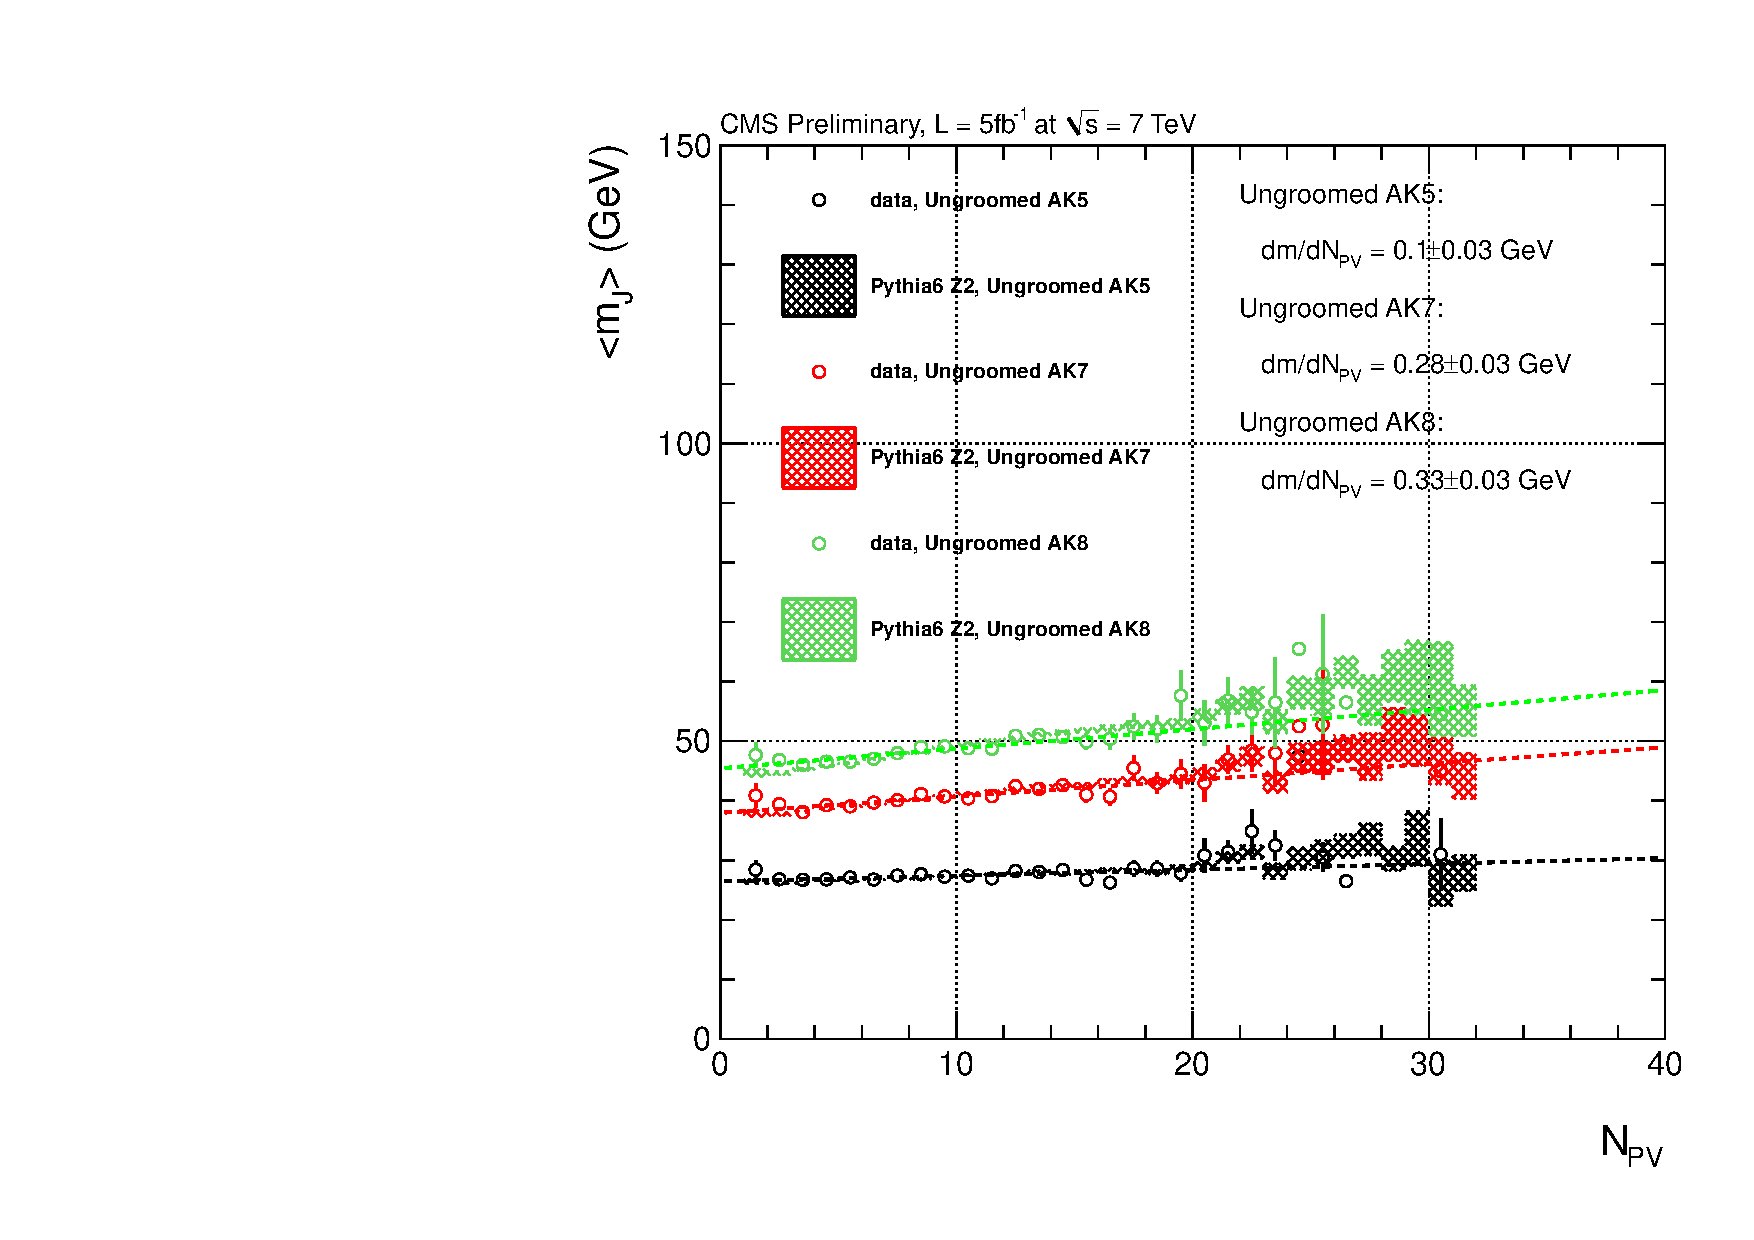
\includegraphics[width=0.495\textwidth]{figs/jetmassproj_vNV_set2.pdf}
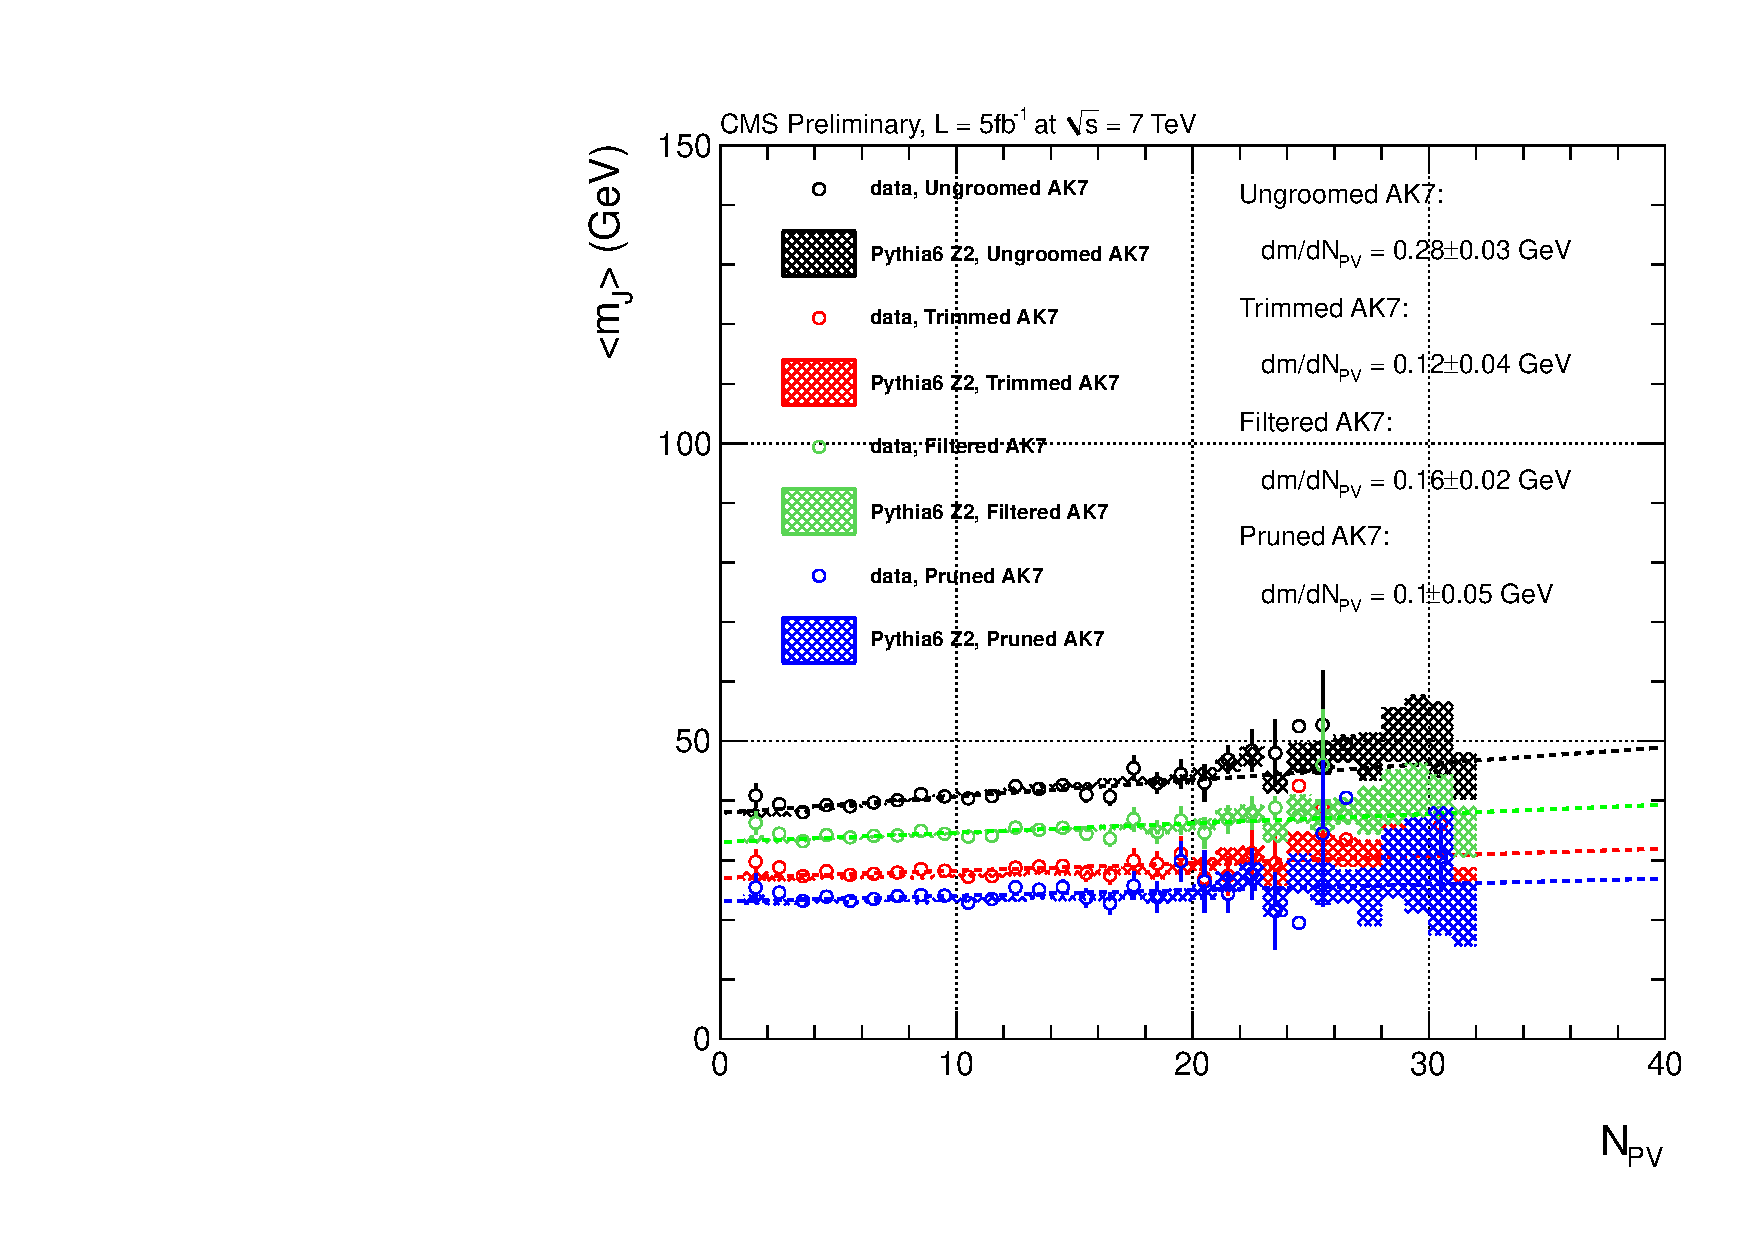
\includegraphics[width=0.495\textwidth]{figs/jetmassproj_vNV_set1.pdf}

\caption{Detector-level distributions of the average jet mass for AK jets, with different radius (left) and for AK7 jets 
for all grooming algorithms as well as the ungroomed distribution (center),
as a function of the number of reconstructed primary vertices.
\label{figs:histAK7MjetVsNvtx_nvtxPlots}}
\end{figure}

\begin{figure}[htbp]
\centering
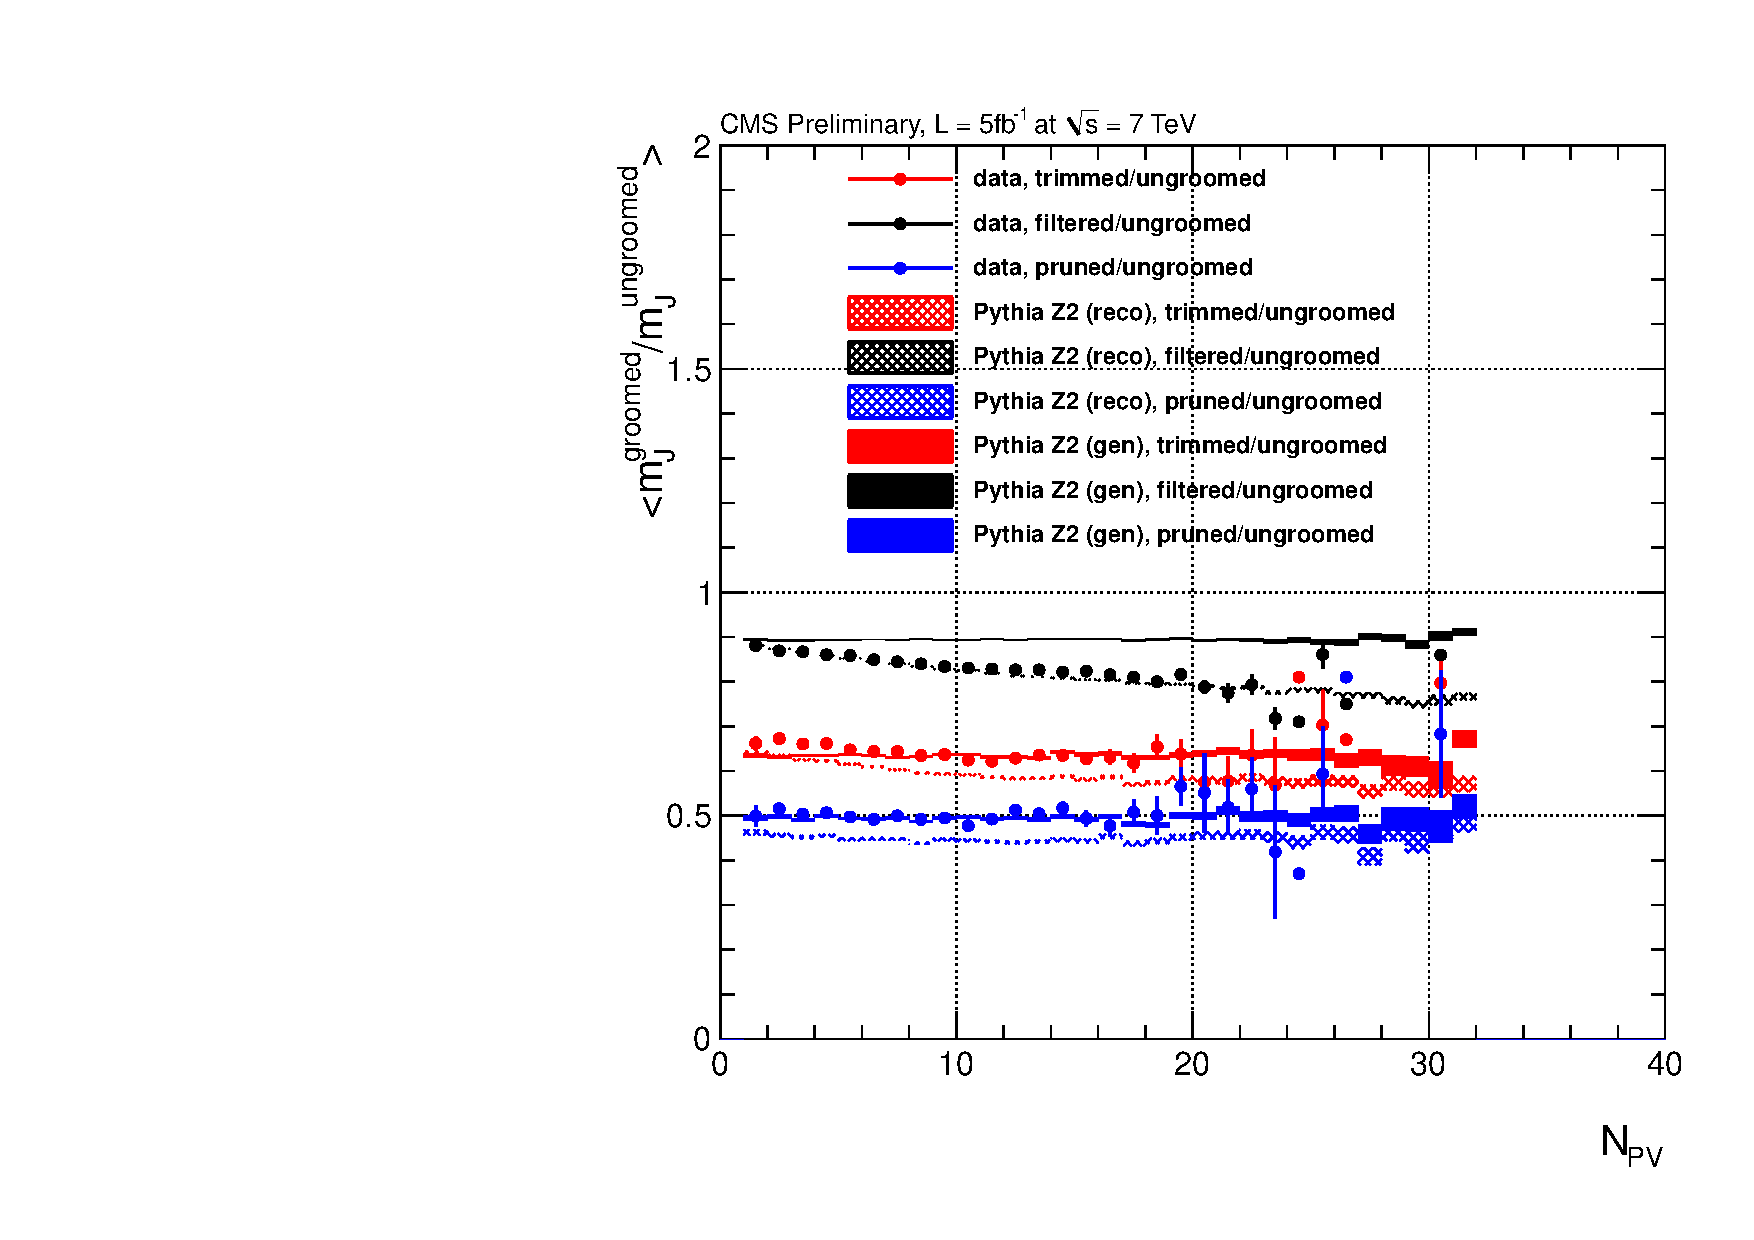
\includegraphics[width=0.495\textwidth]{figs/jetmass_ratioprofileNV_ak7.pdf}

\caption{Detector-level distributions of the average jet mass for groomed AK jets divided by the jet mass of ungroomed jets 
as a function of the number of reconstructed primary vertices. 
\label{figs:histAK7MjetVsNvtx_nvtxPlots2}}
\end{figure}



The excellent data-MC agreement in these distributions as well as the reduced dependence versus pileup for the groomed met mass proves that the pileup dependence of the grooming algorithms is well understood and effective toward pileup suppression.

